\chapter{System implementation}

In this chapter we will discuss the actual implementation of the original idea
behind Linkero: a brand monitoring case management application. We will start
from the architecture in order to show a general snapshot of the system, before
talking in details about every single component, the technology that was
chosen and reasons behind. We will follow with use cases and
system requirements, to conclude with class diagram, database structure and some
code samples.

\section{System architecture}
The system achitecture represented in figure \ref{fig:sysarch} provides an
overview of all different applications that work together to perform the main
system functionalities.

\begin{figure}[h!]
\centering
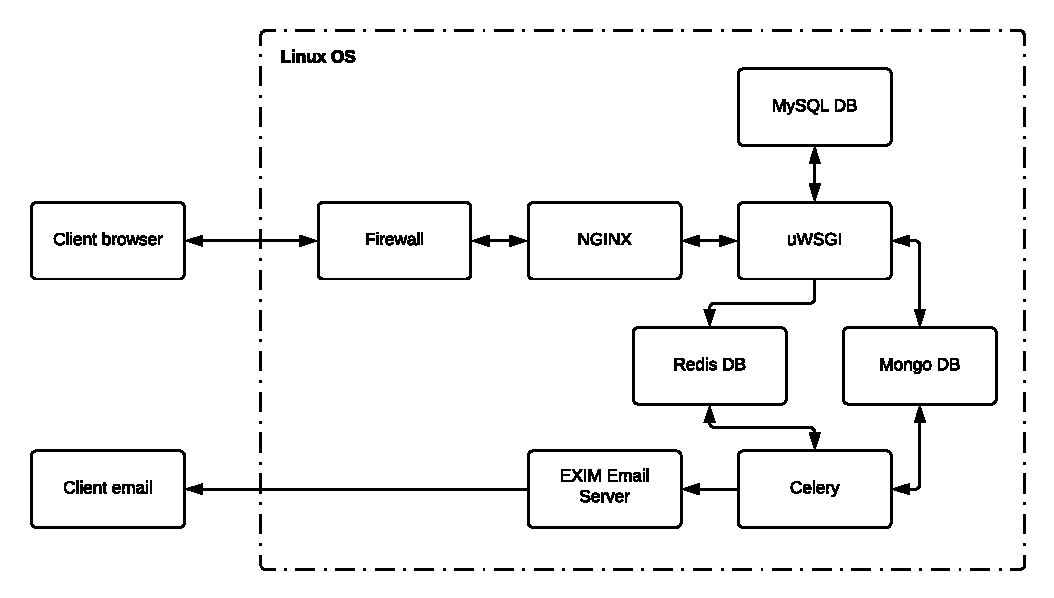
\includegraphics[scale=0.7]{imgs/SystemArchitecture.pdf}
\caption{Linkero system architecture}
\label{fig:sysarch}
\end{figure}

As shown in the figure, client browser and client email are considered part of
the system: the former becuase some functionalities are passed to the client to
run locally in the form of JQuery functions, and the latter because it represent
the final destination of data files generated bythe system.

Linux is the operating system running on a Virtual Private Server, that manages
all other applications. The first point of entry is the Firewall, which monitors
all requests knocking ports 22, 80 and 443.

NGINX is the web server, reverse proxy server \cite{WikiNginx}, which receives
HTTP requests and assigns them to the correct internal web server.

uWSGI is the web engine that runs Python scripts, in the words of its
developers: ``uWSGI itself is a vast project with many components, aiming to
provide a full software stack for building hosting services'' \cite{RtduWsgi}.

Python scripts from within uWSGI can make calls to three databases. MySQL keeps
information about users registration details, passwords, and access logs. Mongo
DB instead is used to store all the data generated by users with their queries.
Finally Redis DB simply stores information about tasks that have been scheduled
and that will run independently from uWSGI's scripts.

Celery is another server running Python scripts scheduled by the main web
server. It does so by regularly checking in Redis if any new task has been
logged, and if that's the case it will execute each task sequentially.

Finally the email server is only called for outgoing emails, to deliver a copy
of all the data collected in a .csv file attached to the email.

\section{Technologies}

The overall system was not written from scratch, there are many free and
open-source applications that were assembled in order for the system to work.

\subsection{Server operating system}
Linkero is hosted on a Virtual Private Server provided by the company Linode
\texttrademark. We chose the smallest package offering 1 GB Ram, 1 CPU Core and
25 GB of SSD storage at \textdollar 5.00 USD a month.

The plan offers different operating systems to chose from, and Linux Debian is
the OS that was picked for this project. There are several advantages to use a
Linux distribution:
\begin{itemize}
  \item Linux is a very lightweight system, which can run on hardware with even
  smaller resources than the ones available for this project;
  \item Linux is mantained by a global community who prioritize reliability and
  security over innovative/experimental functionalities;
  \item Linux is an opesource system, which means that its code can be read by
  anyone, increasing the chances of finding bugs and vulnerabilities, which is
  to say that Linux is very secure;
  \item Linux is also one of the most popular server technologies, guaranteeing
  that a system designed for Linux can access and be transferred to a vast
  public already using Linux;
  \item the Debian distribution development cycle emphasizes stability over
  innovation, offering products that are well tested before being published;
  \item installation and use are free and allowed under the GNU General Public
  License, making it ideal for a small budget project;
  \item the Debian distribution is one of the most rich in extra applications
  ready to be installed from their official directories \cite{Debian}.
\end{itemize}

All the reasons above make Linux Debian the ideal candidate for this project.

\subsection{Web application framework}

As mentioned before, the main business logic in this project is written in
Python and runs on a uWSGI web engine, implementing Python's WSGI convention.
However the actual set of objects and functions that constitute the web application have been developed using Django.
Django is a ``web framework for perfectionists with deadlines'', quoting from
Django developers' tagline \cite{Django}. There are several reasons that make
Django a good candidate for this project:
\begin{itemize}
  \item the web development framework is freely distributed under the BSD
  Licence;
  \item Django offers object-relational mapping classes designed to interact
  directly with a relational database using Python APIs, simplifying
  interactions and data retrival/manipulation operations with a SQL
  database;
  \item Django has already built-in user authentication, authorization and
  session management support, along with a pre-installed admin console with basic
  functionalities. This allows the development process to focus on core
  functionalities, rather than having to code standard session management and
  authentication procedures;
  \item Django comes with several security features to prevent web-specific
  attack, such as: cross-site scripting, cross-site request forgery,
  SQL-injection, clickjacking;
  \item Django is designed with scalability in mind: it enforces strict
  separation between application layer and database layer, so that new hardware
  can be added with no costly impact due to reconfiguration;
  \item successive Django framework versions include backward compatibility and
  try as much as possible to mantain consistent interfaces and API.
\end{itemize}

Chosing Django also means being able to access all the Python libraries
available for data analysis, data mining and system administration.

\subsection{Databases}
There are three different databases that support all the data needs of this
project.

\subsubsection{MariaDB}
MariaDB is a version of MySQL that forket from the original development in order
to remain free under the GNU GPL licence. There is no special reason to prefer
this relational database over the parent MySQL, other than it is the default
version available in the original Debian repositories, since all Debian software
is protected by GNU GPL.

MariaDB is used as default server for user authentication and session
management, and to keep logs of user log-in, user IPs and browsing activity.


\subsubsection{MongoDB}

MongoDB\texttrademark is a NoSQL, schemaless database that stores data in
JSON-like record structures called documents. MongoDB Community Edition is made
available as Debian package under the AGPL licence.

MongoDB is used to store all the data generated while querying external
sources, and is a vital component of the project. The reason for this choice is
simple: MongoDB natural data format is JSON, and does not require the
data schema to be declared in advance. This feature relieves much burden from
the development stage because there is no need to commit to rigid data-schemas
based on the information that are being extracted from external sources, there is
also no need to map a JSON response to a SQL INSERT query. The final
implementation will result in less hard-coded configuration, less maintenance,
more flexibility to accept modification to existing sources and to add new
sources. This doesn't mean that some of the data points extracted should not be
indexed, it actually is recommended to index some crucial data-points to improve
search performance, and MongoDB provides this feature.

There are other features that make MongoDB attractive for this project:
\begin{itemize}
  \item field, range and regulare expressions queries are supported;
  \item results can include user-defined JavaScript functions;
  \item high availability is guaranteed thanks to built-in replication functions
  that make copies of selected data. This feature is relevant if MongoDB is
  deployed across a cluster of multiple machines;
  \item high scalability is also a feature by design;
  \item aggregation can be performed in three different ways, depending on the
  requirement: aggregation pipeline, map-reduce and signle-purpose aggregation
  methods;
  \item finally, as of june 2018, the last version of MongoDB supports full ACID
  transactions.
\end{itemize}

MongoDB does not support SQL style queries, but its query language is very
intuitive, since it reproduces an object-oriented method calling style, for
instance:
\begin{lstlisting}[language=Java, breaklines=true]
db.inventory.find( {
     status: "A",
     $or: [ { qty: { $lt: 30 } }, { item: /^p/ } ]
} )
\end{lstlisting}
in SQL equates to:
\begin{lstlisting}[language=SQL, breaklines=true]
SELECT * FROM inventory WHERE status = "A" AND ( qty < 30 OR item LIKE "p%")
\end{lstlisting}

\subsubsection{Redis}
Finally, the last database implemented in this project is Redis\texttrademark.
The choice of this database was dictated by the need of running an independent
parallel Python thread that would receive requests for specific operations,
and execute them asynchronically from the main web application. A graphical
representation of this asynchronous execution is represented in the sequence
diagram in figure \ref{fig:sqncdiag}. Redis is short for Remote Dictionary
Server, is a database storing key-value data structures in the running
memory, and is distributed under the BSD licence \cite{Redis}. Redis offers the
option to transfer some data to permanent storage, but that is not its strength.
Redis shines in a system with multiple parallel processes that need to
exchange data between each other. Keeping the data in the running memory allows
very quick I/O operations. Also Redis does not support complex queries, and data
aggregate operations, but simple index lookups.

\subsection{Celery}
Celery is an ``asynchronous task queue'' \cite{Celery}, developed in Python and
distributed under the BSD Licence. Celery regularly checks if one or more tasks
are being logged in the Redis database, and executes them in order, while the
main program regains control immediately after submitting a task, so that its
execution is not dependent on the task.

This choice is dictated by two factors:
\begin{itemize}
  \item gathering all the data for one single report can take minutes, or even
  longer, depending on the volume of data requested and the speed of connection.
  In a web application it would result in a bad user experience if the page used
  to submit a report would hang for a long period of time waiting for data to be
  returned.
  \item Services offering API calls to access their data often limit the call
  frequency. Since Linkero is designed to sustain a growing user population,
  we would reach a stange where multiple users could submit concurrent reports,
  and that would likely exceed the API rate limit.
\end{itemize}

In order to solve those two issues, Celery is the central server that receives
and queues all user generated tasks, while executing them one at a time. From
the user perspective, after submitting a report, a feedback message would
acknowledge the fact that the report was submitted successfully, and that a
notification will be sent via email once the report is ready. From the API call
provider perspective, one single agent would make multiple API calls, making
sure not to exceed the limit.

In this configuration, Redis is a message borker that mediates between the web
engine uWSGI and Celery, when tasks are scheduled.

\subsection{Email server}
The email server installed on this system is Exim \cite{exim} which is a very
well established application, first released in 1995 under GNU licence. The
chioce of this server is dictated by the fact that under the current version of
the project a simple send-only email server is sufficient to allow the system to
send out email notification to Linkero users once a report is completed.

\subsection{Web server}
NGINX was chosen to serve the pages of this application. NGINX is an http proxy
and web server \cite{Nginx}, released under the BSD licence.

The main reasons for chosing Nginx over other popular web servers is that its
lighweight even under significant load (2.5MB for 10k simultaneous connections
\cite{wkngx}), and offer native support of WSGI.

There are other reasons that make NGINX a good candidate for the project:
\begin{itemize}
  \item acting as reverse proxy, NGINX adds a layer after the firewall,
  obfuscating the location of web servers, thus improving the system security.
  \item Performs system load balancing when multiple web servers are deployed.
  \item Manages centrally TLS encryption on behalf of every web server under its
  control.
  \item It can host multiple web servers from a single IP.
  \item Finally, it can cache static content, reducing the load to the origin
  servers.
\end{itemize}

\subsection{Firewall}
The firewall application IPtables used in this project comes as default with the
Debian operating system and is distributed freely under the GPL licence
\cite{iptables}. There are no particular reasons why this application was
preferred over others other than:
\begin{itemize}
  \item it is easy to configure;
  \item it is an established application, well documented;
  \item offers filtering at network and transport layers, to provide stateful
  connections inspection.
\end{itemize}

These are the rules implemented for this project:
\begin{itemize}
  \item the default policy on INPUT, FORWARD and OUTPUT chains is to reject
  unless otherwise specified;
  \item block every new incoming request for ports other than 22 (SSH),
  25(SMTP), 80 (HTTP) and 443 (HTTPS);
  \item DROP incoming connections form reserved addresses like (but not limited
  to) 10.0.0.0/8, 169.254.0.0./16, 127.0.0.0/8 or 192.168.0.0/24;
  \item DROP all packets whose state is INVALID;
  \item block for 24 hours IPs that perform portscan;
  \item allow loopback connections;
  \item allow output traffic to ports 22 (SSH), 25 (SMTP), 53 (DNS), 80 (HTTP)
  and 443 (HTTPS).
\end{itemize}

Working along with IPtables, Fail2Ban scans IPtables' log files and dynamically
adds IPtables rules to ban those IPs that behave suspiciously. In
this system installation Fail2Ban is configured to look at SSH login attempts
that fail three times within 24 hours, and bans them for a full day. This
setting targets mainly bots that try to brute-force their way into a server
connected to the public internet, by attempting to login into SSH using a
long list of combinations of username and password. An unusual username and
strong password normally are sufficient to prevent unwanted intrusions, however
leaving the system open to accept and evaluate any volume of login could leave
it exposed to DDoS attacks. Banning activity coming from a suspicious IP is a
way to relieve the pressure from the SSH application, leaving it available to
legitimate users \cite{fail2ban}. As of November 2018, there are currently 603
IPs being banned for a full day, and 8,845 that have been banned at some point
in the last four months of activity.


\section{Development methodology}
For this project, considering its relative simplicity and limited headcount
(one person working on it), Extreme Engineering seemed to be the right
development methodology. The methodology is subdivided into four stages:
planning, design, coding and testing \cite{RP05}. In the next three sections we
will look at the list of requirements and use cases created for this
project, the object oriented class diagrams and some examples of the resulting
code. The next chapter will be dedicated to the testing performed and results.

There are some discrepancies from the XP ortodossy. Extreme programming
encourages for instance to assign priority to each use-case and estimate what is
called \emph{project velocity}, otherwise known as the amount of weeks required
to complete each use-case. With the current level of knowledge, each and every
use-case could be realistically be developed under a week of full time work.
However that did not reflects the reality of time dedicated to each use-case.

Also, extreme programming focusses on the coding part of the development, which
fits the business logic of the project. It is worth to montion that a lot of
time was actually spent configuring off-the-shelf application that constitute
vital parts of the system: enabling NGINX to interact with uWSGI, setting
MongoDB user profiles and credientials, creating an SSL certificate and
registering it in NGINX, and more. All these activities are vital for the
successful implementation and working of the system, but do not feature in the
XP paradigm.


\section{Use cases}
The figure \ref{fig:usecases} represents how the two main end-users types of 
interactions with the system.

\begin{figure}[h!]
\centering
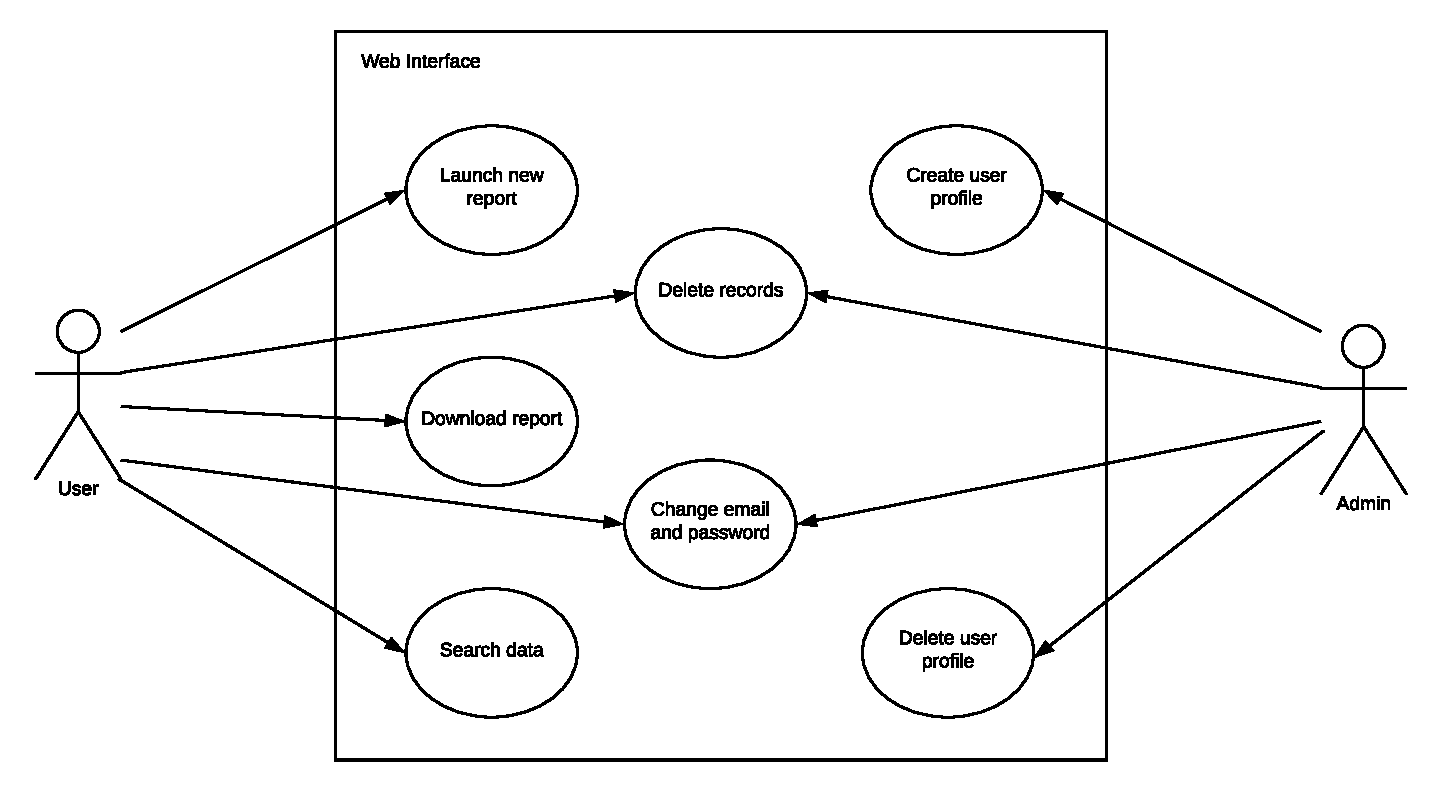
\includegraphics[scale=0.6]{imgs/UseCasesDiag.pdf}
\caption{Use cases diagram}
\label{fig:usecases}
\end{figure}

The figure provides a simplified set of possible actions, with no regard to the
exact order in which they may be presented to the user under realistic
circumstances. Use-cases are a scematic way to visualize the main functions of a
system from the users' perspective.

The follwing set of tables will flash out what each use-case requires and what
provides:

\begin{table}[!h]
\centering
\begin{tabular}{l p{9cm}}  
\toprule
\bf{Use case name}    & Launch new report \\
\midrule
\bf{Actor}    & Investigator \\
\midrule
\bf{Description}    & The user selects the type of report he/she wants to
generate, fills in the necessary input and submits the request. \\
\midrule
\bf{Preconditions}    & The user has to be logged into his/her profile. \\
\midrule
\bf{Trigger}    & Click on \emph{Submit} button. \\
\bottomrule
\end{tabular}
\caption{Launch new report use case}
\end{table}

\begin{table}[!h]
\centering
\begin{tabular}{l p{9cm}}  
\toprule
\bf{Use case name}    & Delete records \\
\midrule
\bf{Actor}    & Investigator, Admin \\
\midrule
\bf{Description}    & The user deletes records associated with a case. \\
\midrule
\bf{Preconditions}    & The user has to be logged into his/her profile. \\
\midrule
\bf{Trigger}    & Click on \emph{Delete} icon. \\
\bottomrule
\end{tabular}
\caption{Delete records use case}
\end{table}

\begin{table}[!h]
\centering
\begin{tabular}{l p{9cm}}  
\toprule
\bf{Use case name}    & Create user profile \\
\midrule
\bf{Actor}    & Admin \\
\midrule
\bf{Description}    & The user create a new profile with a username, email and
password that will allow a new user to access the system functionalities.
\\
\midrule
\bf{Preconditions}    & The user has to be logged into his/her profile. \\
\midrule
\bf{Trigger}    & Click on \emph{Save} button. \\
\bottomrule
\end{tabular}
\caption{Create user profile use case}
\end{table}

\begin{table}[!h]
\centering
\begin{tabular}{l p{9cm}}  
\toprule
\bf{Use case name}    & Download report \\
\midrule
\bf{Actor}    & Investigator \\
\midrule
\bf{Description}    & The user selects a report that has already been
generated, and downloads a csv file with the data.
\\
\midrule
\bf{Preconditions}    & The user has to be logged into his/her profile. Data
from a report has to be already available and saved in the database.
\\
\midrule
\bf{Trigger}    & Click on \emph{Download} icon. \\
\bottomrule
\end{tabular}
\caption{Download report use case}
\end{table}

\begin{table}[!h]
\centering
\begin{tabular}{l p{9cm}}  
\toprule
\bf{Use case name}    & Change email and password \\
\midrule
\bf{Actor}    & Investigator, Admin \\
\midrule
\bf{Description}    & The user can change the current password and email
address.
\\
\midrule
\bf{Preconditions}    & The user has to be logged into his/her profile.
\\
\midrule
\bf{Trigger}    & Click on \emph{Save} button. \\
\bottomrule
\end{tabular}
\caption{Change password use case}
\end{table}

\begin{table}[!h]
\centering
\begin{tabular}{l p{9cm}}  
\toprule
\bf{Use case name}    & Search data \\
\midrule
\bf{Actor}    & Investigator \\
\midrule
\bf{Description}    & The user can submit a set of keywords and find out how
many reports are available in the database associated with that term.
\\
\midrule
\bf{Preconditions}    & The user has to be logged into his/her profile.
\\
\midrule
\bf{Trigger}    & Click on \emph{Search} button. \\
\bottomrule
\end{tabular}
\caption{Search use case}
\end{table}

\begin{table}[!h]
\centering
\begin{tabular}{l p{9cm}}  
\toprule
\bf{Use case name}    & Delete user profile \\
\midrule
\bf{Actor}    & Admin \\
\midrule
\bf{Description}    & The user can delete the profile of a user that no longer
needs access to the system.
\\
\midrule
\bf{Preconditions}    & The user has to be logged into his/her profile.
\\
\midrule
\bf{Trigger}    & Click on \emph{Delete} button. \\
\bottomrule
\end{tabular}
\caption{Delete user profile use case}
\end{table}

\section{Requirements}
We already mentioned some of the requirements and system constraints in the
\emph{system architecture} section. In this section we will discuss in more
details all the requirements considered for the current implementation.
Requirements are further divided in functional, non-functional and user
requirements.

\subsection{Functional requirements}
Functional requirements concerne the core business logic of the system:
\begin{description}
\item[F1] the system should connect successfully to external sources, public
API, to retrieve relevant data.
\item[F2] The system should collect data extracted from external sources and
store it in a local database.
\item[F3] The system should avoid storing duplicates of the same record within
one report request.
\item[F4] The system should assemble all the data gathered for one user's
request and print it in a csv file format.
\item[F5] The system should send a copy of the data, to the requesting user, in
a csv file attached to a notification email.
\item[F6] The system should limit the amount of API calls to each external data
source, in order not to breach API user policy.
\end{description}

\subsection{Non-functional requirements}

\begin{itemize}
  \item security
  \item scalability
  \item maintainability
\end{itemize}

\subsection{User requirements}
\begin{itemize}
  \item 
\end{itemize}

\section{Class diagrams}

\section{Sequence diagrams}

\begin{figure}[h!]
\centering
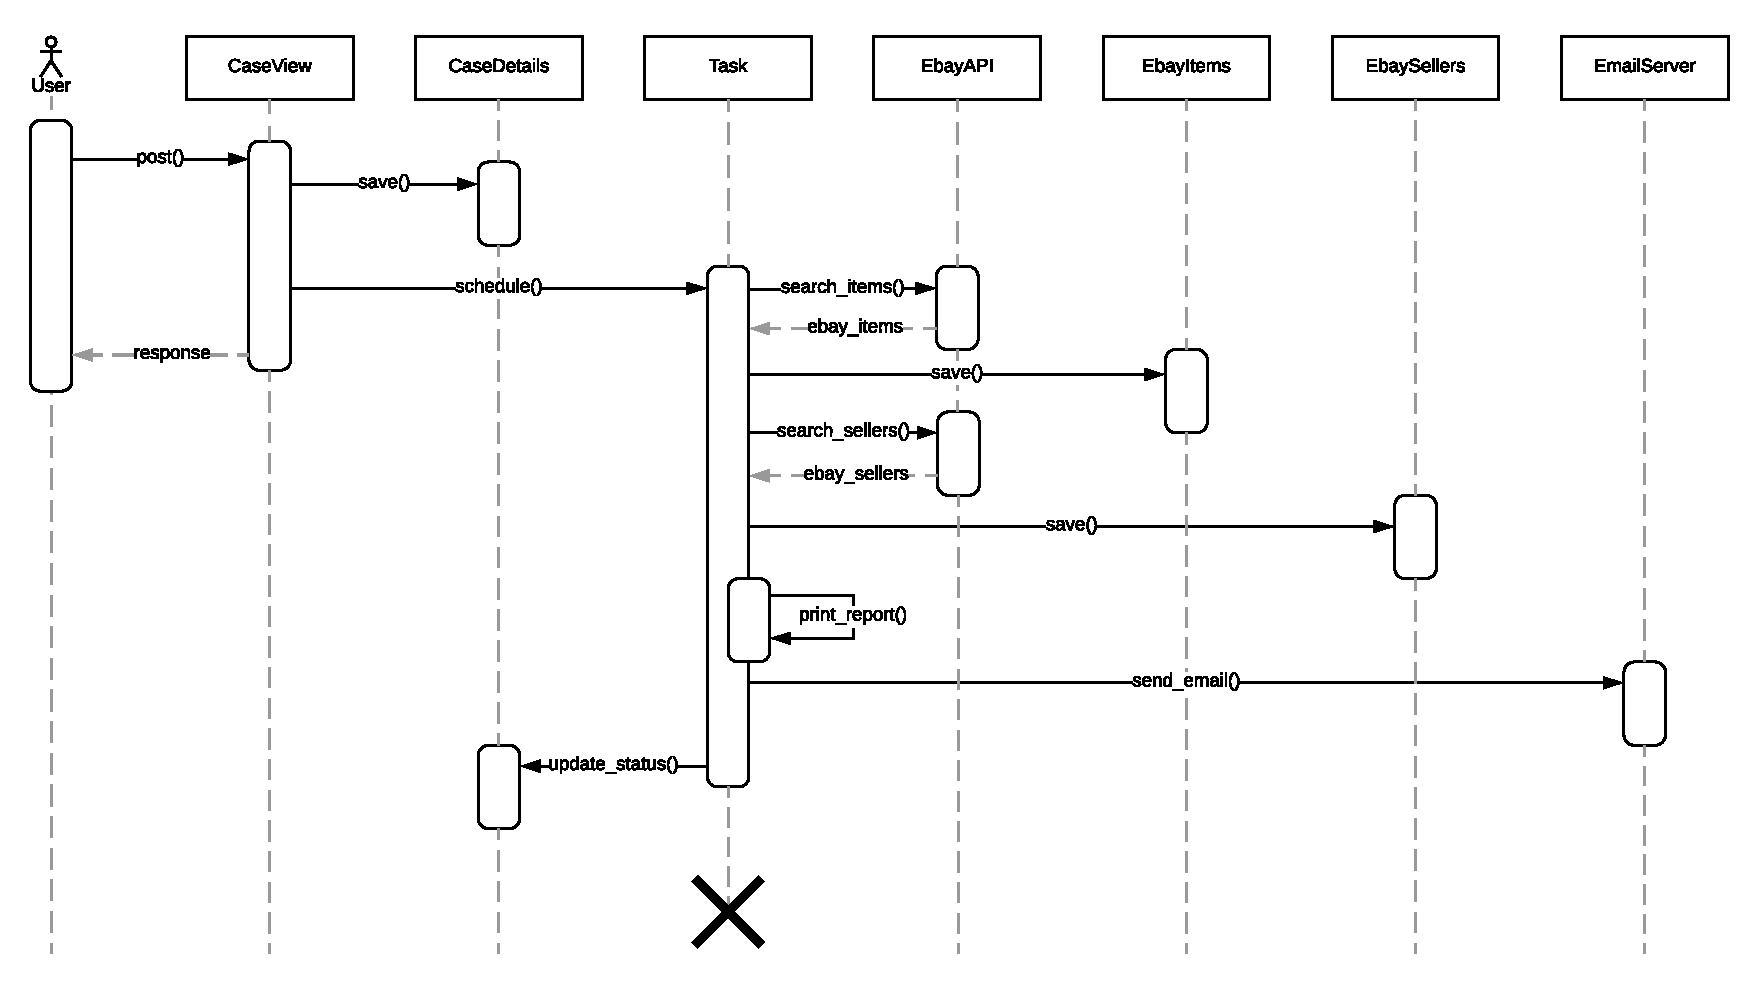
\includegraphics[angle=90, scale=0.6]{imgs/SequenceDiagram.pdf}
\caption{Launch report sequence diagram}
\label{fig:sqncdiag}
\end{figure}

\section{Code samples}
